\documentclass[11pt,reqno]{beamer}
\usepackage[utf8x]{inputenc}
\usetheme{Dresden}
\usecolortheme{beaver}
\usepackage{amsmath}
\usepackage{physics}
\usepackage{amsfonts}
\usepackage{graphicx}
\usepackage{hyperref}
\usepackage{array}   % for \newcolumntype macro
\newcolumntype{R}{>{$}r<{$}}

\setbeamertemplate{navigation symbols}{} 
\title{Bond Graph Clinic: Part 2}
\subtitle{Constitutive Relations}
\author{Peter Cudmore}

\institute{Systems Biology Lab, The University of Melbourne}

\newcommand{\D}[2]{\frac{\mathrm{d} #1}{\mathrm{d} #2}}
\newcommand{\e}{\mathrm{e}}
\newcommand{\I}{\mathrm{i}}
\renewcommand{\mod}[1]{\left|#1\right|}
\newcommand{\DD}[2]{\frac{\mathrm{d}^2 #1}{\mathrm{d} #2^2}}
\newcommand{\bigO}[1]{\text{O}\left(#1\right)}
\renewcommand{\P}[2]{\frac{\partial #1}{\partial #2}}
\renewcommand{\Re}{\operatorname{Re}}
\renewcommand{\Im}{\operatorname{Im}}
\newcommand{\EX}{\mathbb{E}}
\newcommand{\df}[1]{\mspace{2mu}  \mathrm{d}#1}
\newcommand{\reals}{\mathbb{R}}
\newcommand{\complex}{\mathbb{C}}
\newcommand{\conj}[1]{\overline{#1}}

\begin{document}
	\begin{frame}
	\titlepage
	\addtocounter{framenumber}{-1} 
\end{frame}
\begin{frame}
\tableofcontents[hideallsubsections]
\end{frame}
\section{Previously...}
\begin{frame}
\frametitle{Network models of energetic systems}
	\begin{figure}
	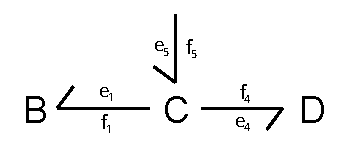
\includegraphics{images/bondgraph.pdf}
\end{figure}
Last week we showed Bond Graphs capture:
\begin{itemize}
	\item Energy transferred between $B,C,D$ without loss via bonds.
	\item Power transfer represented by conjugate variables $P_i=e_if_i$.
	\item Subsystem dynamics through constitutive relations; $\Phi_B(p,q,e,f) = 0$ for example.
\end{itemize}
\end{frame}
\section{Junction Structures}
\subsection{Two-Port Components}
\begin{frame}
\frametitle{Power Conservation Laws}
\begin{figure}
	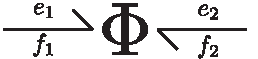
\includegraphics{images/twoport.pdf}
\end{figure}
Suppose this network conserves power, then
\[
e_1f_1 + e_2 f_2 = 0.
\]
That is; the power into $\Phi$ must sum to zero.
Two solutions: $e_1 \propto e_2$, or $e_1\propto f_1$.
\end{frame}
\begin{frame}
\frametitle{Transformer}
\begin{figure}
	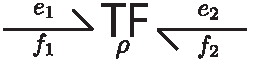
\includegraphics{images/twoport-tf.pdf}
\end{figure}
\only<1>{
\begin{figure}
\begin{minipage}{0.4\linewidth}
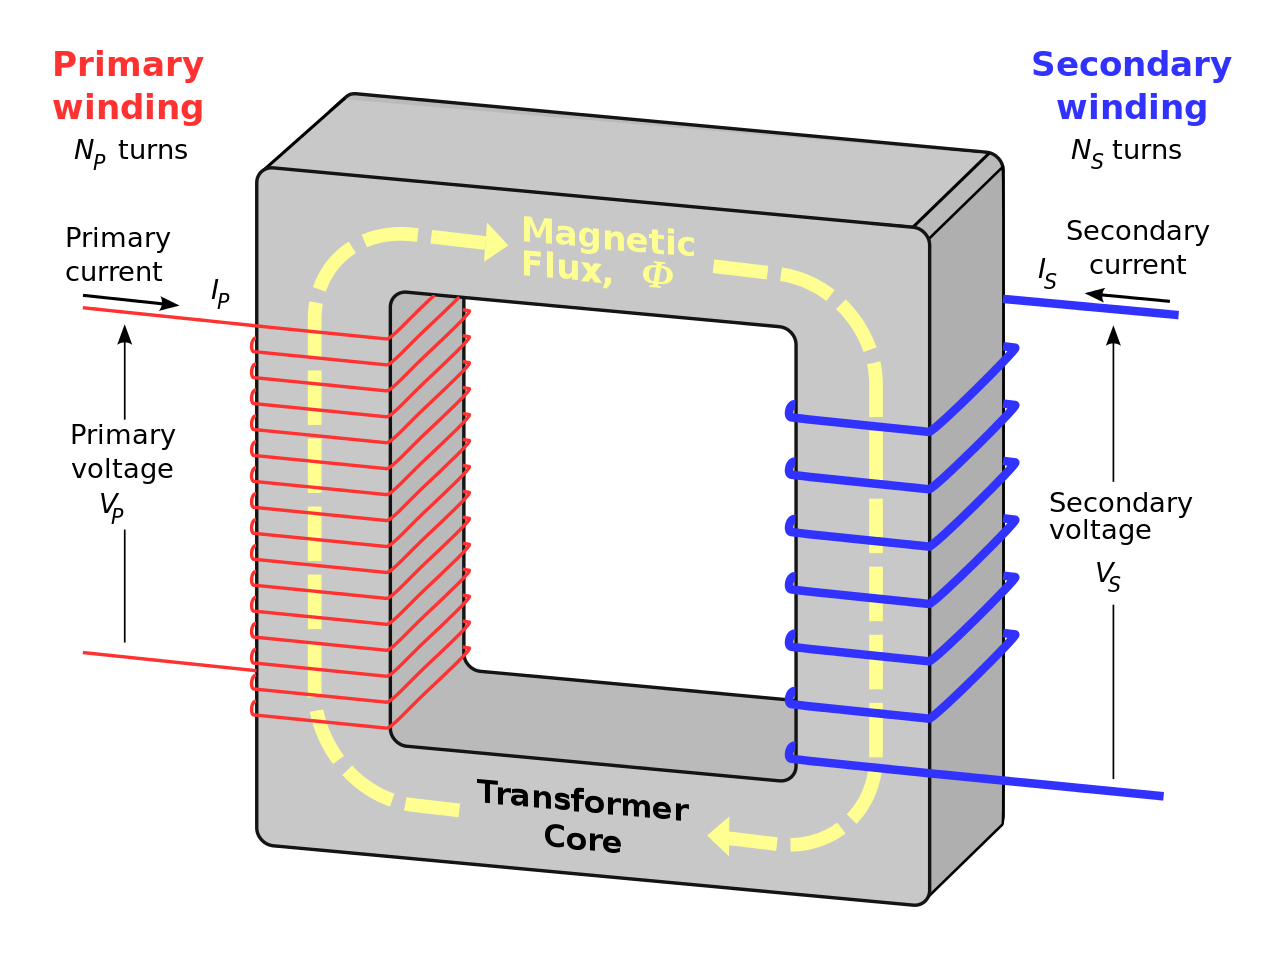
\includegraphics[width=0.8\linewidth]{images/Transformer3d_col.png}
	\end{minipage}
\begin{minipage}{0.4\linewidth}
\raggedright
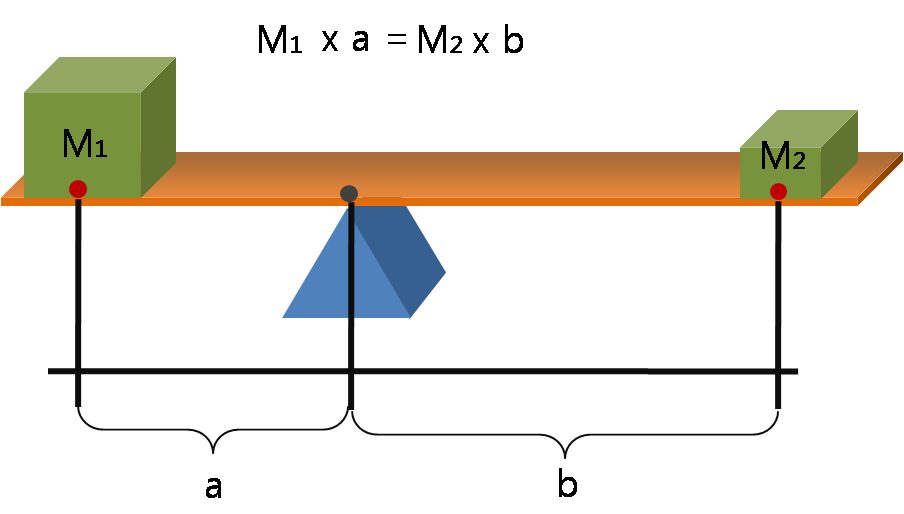
\includegraphics[width=0.8\linewidth]{images/Lever_Principle_3D.png}
\end{minipage}
\caption{An \href{https://en.wikipedia.org/wiki/Transformer}{electrical transformer} and  a \href{https://en.wikipedia.org/wiki/Lever}{mechanical transformer} (ie, a lever)}
\end{figure}
Also includes: motors and generators, waterwheels, etc.
}
\only<2-3>{
For transformers we require $e_2 = \rho e_1$, so 
	\[
e_1f_1 + e_2 f_2 = 0 \implies e_1(f_1 +\rho  f_2)= 0 \implies 
f_2 = -\frac{1}{\rho}f_1
\]
Giving a constitutive relation}
\only<2>{
\[
\Phi_\text{TF} =\left(\begin{matrix}
e_2 - \rho e_1 \\
f_2 +\frac{1}{\rho}f_1
\end{matrix} \right)  = 0.
\]}
\only<3>{
	\[
	\Phi_\text{TF} = \left(
	\begin{matrix}
	-\rho & 0  &1 &  0 \\
	0&\rho^{-1} &0  & 1 
	\end{matrix}\right)
	\left(\begin{matrix}
e_1\\
f_1\\
e_2\\
f_2
	\end{matrix}
	\right) = 0.
	\]
}
\end{frame}
\begin{frame}
\frametitle{Gyrator}
\begin{figure}
	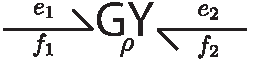
\includegraphics{images/twoport-gy.pdf}
\end{figure}
\only<1>{
\begin{figure}
	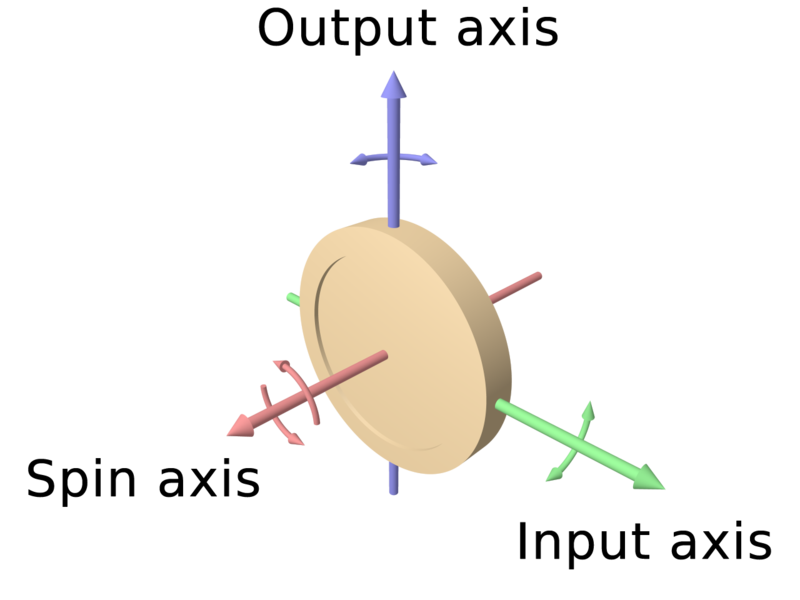
\includegraphics[width=0.3\linewidth]{images/Gyroscope.png}
	\caption{\href{https://en.wikipedia.org/wiki/Gyroscope}{A gyroscope}}
	\end{figure}
Electrical gyrators were proposed by Tellengen in 1948, but a passive implementation hasn't yet been found.
}
\only<2-3>{
For gyrators we require $e_2 = \rho f_1$, so
\[
e_1f_1+e_2f_2 = 0 \implies  f_1(e_1 -  \rho f_2)=0 \implies f_2 = -\frac{1}{\rho}e_1.
\]
Giving a constitutive relation}
\only<2>{
\[
\Phi_\text{GY} =\left(\begin{matrix}
e_2 - \rho f_1 \\
f_2 +\frac{1}{\rho}e_1
\end{matrix} \right)  = 0.
\]}
\only<3>{
\[
\Phi_\text{GY} = \left(
\begin{matrix}
0 & -\rho  &1 &  0 \\
\rho^{-1}&0 &0  & 1 
\end{matrix}\right)
\left(\begin{matrix}
e_1\\
f_1\\
e_2\\
f_2
\end{matrix}
\right) = 0.
\]
}

\end{frame}
\subsection{N-port Components}
\begin{frame}
\frametitle{Network Conservation Laws}
\begin{figure}
	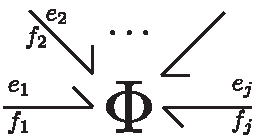
\includegraphics{images/nport.pdf}
\end{figure}
We require nodes to capture the distribution of power across many subsystems. These junction nodes capture network conservation laws which must satisfy
\[
0 = \sum_{i=1}^j e_if_i.
\]
The two base cases are \emph{common effort}, and \emph{common flow}.
\end{frame}
\begin{frame}
\frametitle{0-Junction}
\begin{figure}
	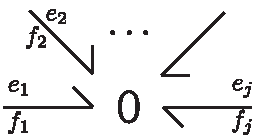
\includegraphics{images/nport-0.pdf}
\end{figure}
\only<1>{
For common effort junctions $e_i = e_k,\ \forall 1\le i,k \le j$. Hence
\[
\sum_{i=1}^j e_i f_i = 0 \implies  \sum_{i=1}^j f_i = 0
\]
\emph{This is Kirchoff's Current Law}
}
\only<2>{
The constitutive relation is given by:
\[
\Phi_\text{0} = \left(\begin{matrix}
e_1 -e_2\\
\ldots\\
e_{j-1} - e_j\\
f_1 + f_2 + \ldots + f_j 
\end{matrix}\right) = 0
\] 
}
\only<3>{
	The constitutive relation is given by:
	\[
	\Phi_\text{0} = \left(\begin{matrix}
1 	& 0		   & -1		& 0 	& 	\ldots &0 \\
&	 \ddots& & \ddots  & \\
\ldots  & 0  & 	  1   & 0         & -1 &0\\
      0 & 1 & \ldots & & 0 &1
	\end{matrix}
	\right)
	\left(\begin{matrix}
e_1\\f_1\\\vdots\\ e_j\\f_j
	\end{matrix}\right)
	 = 0
	\] 
}
\end{frame}
\begin{frame}
\frametitle{1-Junction}
\begin{figure}
	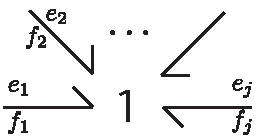
\includegraphics{images/nport-1.pdf}
\end{figure}
\only<1>{
Similarly for common flow junctions $f_i = f_k,\ \forall 1\le i,k \le j$. Hence
	\[
	\sum_{i=1}^j e_i f_i = 0 \implies  \sum_{i=1}^j e_i = 0
	\]
	\emph{This is Kirchhoff's Voltage Law}
}
\only<2>{
	The constitutive relation is given by:
	\[
	\Phi_\text{1} = \left(\begin{matrix}
	f_1 -f_2\\
	\ldots\\
	f_{j-1} - f_j\\
	e_1 + e_2 + \ldots + e_j 
	\end{matrix}\right) = 0
	\] 
}
\only<3>{
	The constitutive relation is given by:
	\[
	\Phi_\text{1} = \left(\begin{matrix}
	0 	& 1		   &0		& -1 	& 	\ldots &0 \\
&	&	 \ddots& & \ddots   \\
	\ldots  & & 0  & 	  1   & 0         & -1\\
	1 & 0 & \ldots & & 1 &0
	\end{matrix}
	\right)
	\left(\begin{matrix}
	e_1\\f_1\\\vdots\\ e_j\\f_j
	\end{matrix}\right)
	= 0
	\] 
}\end{frame}
\section{Storage and I/O}
\subsection{Storage}
\begin{frame}
\frametitle{Physics review}
Energy stored is a function of local storage co-ordinates $q,p$
\[
H(q, p) = E_0 + \int P_\text{in}\df{t}.
\]
The canonical co-ordinates $q, p$ are taken such that $q \in X$ where $X$ is some manifold, and $p\in X^*$ where $X^*$ is the dual space of $X$. 
\vspace{10pt}

In the case where $X = \mathbb{R}^n$, the dual space $X^*$ is the set of column vectors acting on $X$.
That is if $q,x \in \mathbb{R}^n$ then there exists a dual vector (a linear functional) $p \in X^*$ such that $p(q) = x^T\cdot q$.

\vspace{10pt}

As an aside, in physics $p$ is often written as $\bra{p}$, so that in the above example $\bra{p}\ket{q} = x^Tq$.
\end{frame}

\begin{frame}
\frametitle{Physics review (cont.)}
If $P_\text{in} = ef$ then
\[
H(q, p) = E_0 + \int P_\text{in}\df{t} \implies \P{H}{q} \df{q} + \P{H}{p}\df{p} = ef\df{t}.
\]
We want to:
\begin{itemize}
	\item associate $e$ with the tangent space of $X^*$, ideally by saying something like $e = \D{p}{t}$ so that $e\df{t} =\df{p}$.
	\item associate $f$ with the tangent space of $X$, ideally by saying that $f = \D{q}{t}$ so that $f\df{t} = \df{q}$.
\end{itemize}
We can do this easily if we consider individual components whose stored energy depends only on generalised position or momentum, but not both.
\end{frame}
\begin{frame}
\frametitle{Kinetic Storage}
\begin{figure}
	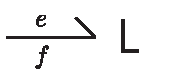
\includegraphics{images/oneport-L.pdf}
\end{figure}
For kinetic energy, the stored energy depends only on momentum, $\P{H}{q} = 0$, so we can define $e\df{t} = \df{p}$.
\[
\P{H}{q} \df{q} + \P{H}{p}\df{p} = ef\df{t} \implies  \left(\P{H}{p} - f\right)\df{p}= 0
\]
Hence we have a constitutive relation
\[
\Phi_L = \P{H}{p} - f= 0, \qquad  \text{where}\qquad \dot{p} = e.
\]
\end{frame}
\begin{frame}
\frametitle{Kinetic Storage (cont.)}
\begin{figure}
	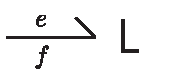
\includegraphics{images/oneport-L.pdf}
\end{figure}
\only<1>{
In the case of linear kinetic storage; we have a Hamiltonian
\[
H(q,p) = \frac{1}{2L}p^2,
\]
which is the energy stored in a $L$-henry inductor; in the linear motion of an $L$-kg object.\\

\vspace{10pt}
This gives rise to the familiar constitutive relation:
\[
\Phi_L = \P{H}{p} - f = \frac{1}{L}p - f\qquad \implies \qquad Lf -  \int e \df{t} = 0.
\]}
\only<2>{
This gives rise to the familiar constitutive relation:
\[
\Phi_L = \frac{1}{L}p - f
\]
Which, if we define the integration operator $\mathcal{I}x = \int_0^tx(t)\df{t}$, then we have
\[
\Phi_L = \left(\mathcal{I}, -L\right) \left(\begin{matrix} e\\f\end{matrix}\right) \qquad \overset{\mathcal{L}}{\implies}\qquad
\hat{\Phi}_L(s) = \left(s^{-1}, -L\right) \left(\begin{matrix} \hat{e}\\\hat{f}\end{matrix}\right) 
\] 
}
\end{frame}

\begin{frame}
\frametitle{Potential Storage}
\begin{figure}
	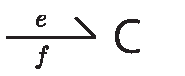
\includegraphics{images/oneport-C.pdf}
\end{figure}
Similarly for potential, the stored energy depends only on position, $\P{H}{p} = 0$, so we define $f\df{t} = \df{q}$.
\[
\P{H}{q} \df{q} + \P{H}{p}\df{p} = ef\df{t} \implies  \left(\P{H}{q} - e\right)\df{q}= 0
\]
Hence we have a constitutive relation:
\[
\Phi_C = \P{H}{q} - e= 0, \qquad  \text{where}\qquad \dot{q} = f.
\]
\end{frame}

\begin{frame}
\frametitle{Potential Storage (cont.)}
\begin{figure}
	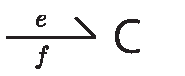
\includegraphics{images/oneport-C.pdf}
\end{figure}
\only<1>{
Storage of potential energy has more variety. In the linear case (represented by the $C$ node above) we have
\[
H(q,p) =\frac{1}{2C} q^2 
\]
which is the power stored in a $C$-farad capacitor, the elastic energy stored in a spring displaced by $q$ from equilibrium, etc.
\[
\Phi_C = \P{H}{q} - e= \frac{1}{C}q - e \qquad  \implies \qquad Ce - \int f \df{t} = 0
\]}
\only<2>{
Hence we have a constitutive relation:
\[
\Phi_C = \frac{1}{C}q - e
\]
Which, if we define the differentiation operator $Dx = \D{}{t} x(t) $, then we have
\[
\Phi_C = \left(C, -D\right) \left(\begin{matrix} e\\f\end{matrix}\right) \qquad \overset{\mathcal{L}}{\implies}\qquad
\hat{\Phi}_C(s) = \left(C, -s\right) \left(\begin{matrix} \hat{e}\\\hat{f}\end{matrix}\right) 
\] 
up to a constant.
}
\end{frame}

\subsection{Dissipative and Sources}
\begin{frame}
\frametitle{Linear Dissipation}
\begin{figure}
	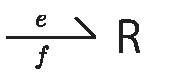
\includegraphics{images/oneport-R.pdf}
\end{figure}
Dissipation can be captured by introducing a Dirac structure $\mathcal{D}(\dot{q})$, and choosing $f = \dot{q}$ such that
\[
\mathcal{D}(\dot{q})\df{q} = e\df{q} \implies \Phi_R = e - \mathcal{D}(f) =0\]
Clearly picking $\mathcal{D}(\dot{q}) = R\dot{q}$ gives both Ohms law and friction so that
\[
\Phi_R = e - Rf = 0
\]
\end{frame}

\begin{frame}
\frametitle{Effort and Flow sources}

\begin{figure}
	\begin{minipage}{0.4\textwidth}
	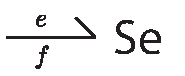
\includegraphics{images/oneport-Se.pdf}
	\end{minipage}
	\begin{minipage}{0.4\textwidth}
	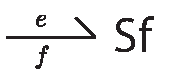
\includegraphics{images/oneport-Sf.pdf}
\end{minipage}
\end{figure}
To get power in and out of the system, we add control nodes. These impose a control value $u(t)$ on $e$ (for Se) or $f$ (for Sf), and leave the other variable free, under the assumption that there is enough power on tap to maintain the control value. 
For the effort source Se we have
\[
\Phi_\text{Se} = e - u.
\]
and similarly for the flow source Sf
\[
\Phi_\text{Sf} = f - u.
\]
\end{frame}
\section{An example...}
\begin{frame}
\frametitle{Table of Constitutive Relations}
\begin{small}
\begin{minipage}[c][\textheight][t]{0.4\textwidth}
\vspace{0.75cm}
\begin{tabular}{| l | c |}
	Node & Constitutive Relation\\
	\hline
	& \\
	R & $\Phi_\text{R} = e -Rf$\\
	L & $\Phi_\text{L} = \int e\df{t} - Lf$\\
	C & $\Phi_\text{C} = Ce - \int f \df{t}$\\
	Se & $\Phi_\text{Se} = e - u$\\
	Sf & $\Phi_\text{Sf} = f - u$\\
	TF & $\Phi_\text{TF} =\left(\begin{matrix}
	e_2 - \rho e_1 \\
	f_2 +\frac{1}{\rho}f_1
	\end{matrix} \right)$\\
	GY & $\Phi_\text{GY} =\left(\begin{matrix}
	e_2 - \rho f_1 \\
	f_2 +\frac{1}{\rho}e_1
	\end{matrix} \right)$
\end{tabular}
\end{minipage}\hfill
\begin{minipage}[c][\textheight][t]{0.45\textwidth}
	\vspace{0.75cm}
\begin{tabular}{| l | c |}
	Node & Constitutive Relation\\
	\hline
	&\\
	0 &$	\Phi_\text{0} = \left(\begin{matrix}
	e_1 -e_2\\
	\ldots\\
	e_{j-1} - e_j\\
	f_1 + f_2 + \ldots + f_j 
	\end{matrix}\right)$\\
	&
	\\
	1&$	\Phi_\text{1} = \left(\begin{matrix}
	f_1 -f_2\\
	\ldots\\
	f_{j-1} - f_j\\
	e_1 + e_2 + \ldots + e_j 
	\end{matrix}\right)$
\end{tabular}
\end{minipage}
\end{small}
\end{frame}
\begin{frame}
\frametitle{RLC Example}
\begin{small}
\begin{minipage}{0.4\textwidth}
\begin{figure}
	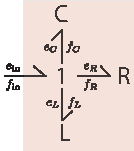
\includegraphics{images/rlc.pdf}
	\caption{RLC Bond Graph}
\end{figure}
\end{minipage}
\begin{minipage}{0.55\textwidth}
\begin{eqnarray}
\Phi_R &=& e_R - Rf_r\\
\Phi_C &=& Ce_C - \int f_C\df{t}\\
\Phi_L &=& \int e_L \df{t} - Lf_L\\
\Phi_1 &=& \left(\begin{matrix}
f_\text{in} - (-f_R)\\
f_\text{in} - (-f_C)\\
f_\text{in} - (-f_L)\\
e_\text{in} + e_R + e_C + e_L
\end{matrix}\right)
\end{eqnarray}
\end{minipage}


\vspace{10pt}

\only<1>{Our goal is to find $\Phi_\text{RLC}(e_\text{in},f_\text{in}) = 0$; that is the equivalent relation for the entire network.}
\only<2>{Observing the first three rows of $\Phi_1$, in combination with $\Phi_R,\Phi_C,\Phi_L$ respectively; we have
	\[
	e_R = -Rf_\text{in},\qquad e_c = -\frac{1}{C}\int f_\text{in}\df{t}, \qquad e_L = -\frac{1}{L}\D{f_\text{in}}{t}
	\]
}
\only<3>{
Substituting into the fourth row of $\Phi_1$ gives our result:
\[
\Phi_\text{RLC} = e_\text{in} - \left(\frac{1}{C}\int f_\text{in} \df{t} + Rf_\text{in} + \frac{1}{L}\D{f_\text{in}}{t}\right) = 0
\]
}
\end{small}
\end{frame}
\end{document}